\documentclass[a4paper]{article}
\usepackage{amsmath, amssymb}
\usepackage[swedish]{babel}
\usepackage{graphicx}
\graphicspath{{imgs/}}
\usepackage{float}
\usepackage[hidelinks]{hyperref}
\usepackage{fancyhdr}
\usepackage[parfill]{parskip}
\usepackage[margin=1in]{geometry}
\usepackage{listings}
\usepackage{xcolor}
\usepackage[style=ieee, backend=biber]{biblatex}
\usepackage{csquotes}
\addbibresource{../sources.bib}
\setcounter{secnumdepth}{0}
\pagestyle{fancy}
\fancyhf{}
\setlength{\headheight}{12.31253pt}
\newcommand{\getauthor}{Eric Johansson (erjo2002@student.miun.se)\\
                        Can Kupeli (caku2002@student.miun.se)\\
                        Samuel Greenberg (sagr1908@student.miun.se)} %Author
\newcommand{\gettitle}{Laboration 3 \\ Markovkedjor och Köteori} %Title
\newcommand{\getcourse}{(MA069G, Matematisk Modellering, 6hp)} %Course
\newcommand{\getsupervisor}{Magnus Eriksson}


\definecolor{codegreen}{rgb}{0,0.6,0}
\definecolor{codegray}{rgb}{0.5,0.5,0.5}
\definecolor{codepurple}{rgb}{0.58,0,0.82}
\definecolor{backcolour}{rgb}{0.95,0.95,0.92}

\lstdefinestyle{mystyle}{
    backgroundcolor=\color{backcolour},   
    commentstyle=\color{codegreen},
    keywordstyle=\color{magenta},
    numberstyle=\tiny\color{codegray},
    stringstyle=\color{codepurple},
    basicstyle=\ttfamily\footnotesize,
    breakatwhitespace=false,         
    breaklines=true,                 
    captionpos=b,                    
    keepspaces=true,                 
    numbers=left,                    
    numbersep=5pt,                  
    showspaces=false,                
    showstringspaces=false,
    showtabs=false,                  
    tabsize=2
}

\lstset{style=mystyle}

\begin{document}

\begin{titlepage}
  \begin{center}
    \vspace*{1cm}
    
\includegraphics[width=0.8\textwidth]{msu.png}\\[0.5cm]
    \Large
    Institutionen för matematik och ämnesdidaktik (MOD)\\[1cm]
    \Huge
    \textbf{\gettitle}

    \large
    \getcourse{}

    \vspace{1cm}
    \getauthor{}
    \vfill
    \vspace{0.8cm}
    \small
    \today \\
    \Large
    \textbf{Handledare:}\\
    \getsupervisor{}
  \end{center}
\end{titlepage}

\lhead{Laboration 3}
\rhead{Markovkedjor och Köteori}
\tableofcontents
\newpage

\section{Förord}
Denna laboration ger er möjlighet att bekanta er Markovkedjor och köteori
och hur man kan använda Python för att beräkna stationära sannolikheter.

Det rekommenderas att ni använder er av verktyget Jupyter Notebooks för att lösa
uppgifterna. I det verktyget kan man sammanställa block med Python-kod, beräkningsresultat,
plottar och egen text med ekvationer i ett och samma dokument, och köra all kod i dokumentet
i följd eller interaktivt. Jyputer Notebook ingår i utvecklingsmiljön Anaconda, som du med
fördel kan välja att installera och använda, eftersom den innehåller Pythonbibliotek och
verktyg som är vanliga inom beräkningsvetenskap, datamining och maskininlärning, och som passar ihop.

För att utföra laborationen rekommenderas det att biblioteken numPy \cite{numpy-main},
symPy \cite{sympy-main} och matplotlib \cite{matplotlib-main} används. De är inkluderade i Anaconda men kan annars installeras genom att
skriva ``pip install \textit{namn}'' i terminalen i Windows eller ``pip3 install \textit{namn}'' på Mac eller Linux.
För många vanliga matematiska funktioner som till
exempel sinus, kvadratroten och log kan det krävas att ni importerar math-biblioteket i er skript men generellt kan numPys
verisioner av dessa funktioner användas istället.

\textbf{Instruktionerna kommer utgå ifrån att ni har skrivit detta i början av er fil / notebook}
\begin{lstlisting}[language=Python]
import math 
import numpy as np
import sympy as sy
from matplotlib import pyplot as plt
\end{lstlisting}

Därefter kan ni använda funktionaliteten från de olika biblioteken genom att
kalla deras funktioner. Exempelvis math.sqrt(), np.cos(), sy.symbols()

I rapporten skall ni bifoga er kod, beräkningsresultat, diagram, korta svar och förklaringar.
Allas namn och datum måste ingå i dokumentet.

\newpage
\section{Uppgift 1: Iterativ numerisk beräkning}
Man har genom att studera den finansiella marknaden under en längre tid funnit ett samband mellan vad som kallas Bull, Bear samt Recession.

En marknad är i Bull då man förväntar sig en uppgång, Bear om man föväntar en nedgång och är det riktigt dåligt har vi Recession, vilket ofta sammanfaller
med en omväröd i gunging som t.ex. vid finanskrisen 2008.

Sambandet under en given vecka illustreras i Figur \ref{fig:bbr}

\begin{figure}[H]
  \centering
  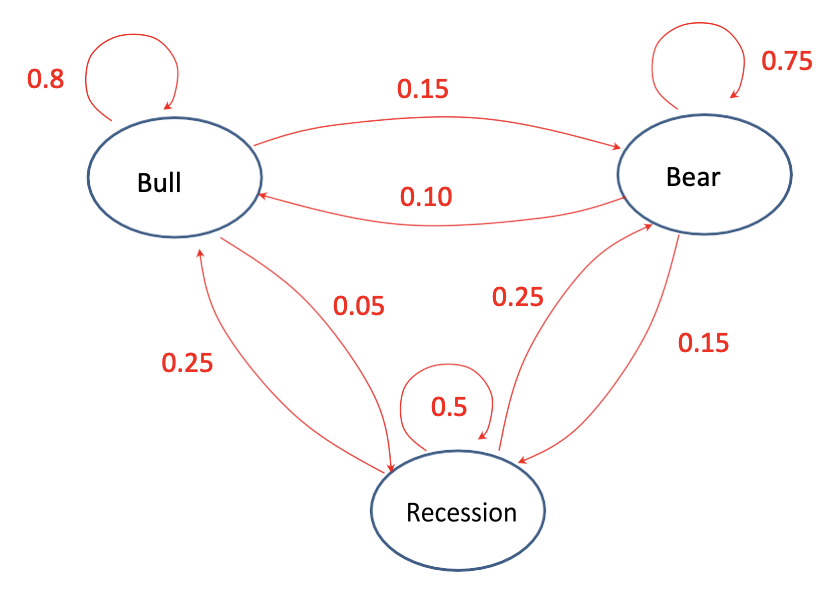
\includegraphics[width=0.8\textwidth]{bbr.png}
  \caption{Rådande marknadssituation under en given vecka}
  \label{fig:bbr}
\end{figure}

Från Figur \ref{fig:bbr} kan man räkna ut hur fördelningen kan väntas vara på lång sikt gällande Bull, Bear samt Recession.
Detta kan vara till hjälp för de som investerar i marknaden.

\subsection{a)}
Sätt upp överföringsmatrisen \( P \) för problemet i Figur \ref{fig:bbr} så att radsumman blir 1.

\subsection{b)}
Anta en startvektor (radvektor) och en toleransnivå samt gör ett program som iterativt
beräknar hur tillståndssannolikheterna konvergerar mot en stationär lösning. Beskriv den
metod du har valt för att beräkna det fel som jämförs med toleransnivån; är det en ett-norm
(summan av absolutbeloppen av felen), två-norm (roten ur medelvärdet av kvadratiska
felen) eller oändlighetsnorm (max av absolutbeloppen)?

\subsection{c)}
Ange stationära lösningen samt hur många iterationer det tar till den når lösningen vid en
viss toleransnivå.

\subsection{d)}
Har startvektorn betydelse för det stationära resultatet, dvs är det en icke-ergodisk process?

\subsection{e)}
Har startvektorn betydelse för konvergenstiden? Vilken startvektor ger isåfall snabbast
lösning, inom en iteration?

\section{Uppgift 2: Exakt beräkning}
Verifiera svaret i Uppgift 1 genom att lösa ekvationer för stationära sannolikheter
(ett egenvärdesproblem), genom att sätta nuvarande tillstånd lika med nästa tillstånd, och
kombinera det med att summan av sannolikheterna ska bli 1. Använd gärna flera metoder: Du
kan handräkna med insättningsmetoden eller gausselimination,
använda np.linalg.lstsq(), utnyttja sympy.stats.DiscreteMarkovChain eller använda
webbplatsen Wolfram Alpha.

\textbf{Svara på följande frågor i rapporten}

Vad är det exakta värdena?


\section{Uppgift 3: Stokastisk simulering}
Skapa en stokastisk simulering (Monte Carlo-simulering) av Markovkedjan med hjälp av
slumptalsgenerering och metoden inverse transform sampling. Slumpa ett starttillstånd \( k \) som
talen 1, 2 eller 3, eventuellt baserat på en startvektor. Om nuvarande tillstånd är \( k \), anges
sannolikheterna för nästa tillstånd av rad \( k \) i övergångsmatrisen, dvs av P[k,:] i Pythonkod.
Beräkna tillståndens frekvenser som f(k)=f(k)+1. De relativa frekvenserna f/np.sum(f)
konvergerar mot den stationära fördelningen.


\textbf{Svara på följande frågor i rapporten}

Ungefär hur många iterationer tar det innan
tillståndens frekvenser konvergerar mot en stationär lösning med rimlig noggrannhet?

Är detta snabbare eller långsammare än metod 1?


\section{Uppgift 4: Markov-egenskapernas betydelse}
Genom att ändra lite i övergångssannolikheterna i Figur 1 kan man analysera hur den
stationära lösningen ändras. Ge exempel på en förändring av sannolikheterna som skulle ge
en icke-ergodisk process och därmed inte skulle ge stationär lösning oberoende av
initialtillståndet, dels

\subsection{a)}
i form av en periodisk (cyklisk, deterministisk) kedja, dels

\subsection{b)}
en reducivel stokastisk process där alla tillstånd inte kommunicerar, och den stationära
lösningen därför beror av initialtillsåndet.

\subsection{c)}
Ge även exempel på en icke-minnesfri process genom att införa villkor i tillståndsdiagrammet.

\subsection{d)}
Diskutera för vilka av dessa processer (som inte uppfyller Markov-egenskaperna) som den
stationära sannolikheten för valfri startvektor potentiellt skulle kunna beräknas med
metoderna i uppgift 1, 2 respektive 3. I vilka fall måste metoden i uppgift 1 och 3 kompletteras
med en yttre loop som slumpar flera olika starttillstånd, och beräknar ensemblemedelvärdet
av de olika utfall som då erhålles?

\newpage
\section{Uppgift 5: Kösystem}
Betrakta en liten butik med plats för fyra kunder. Den kan vara i fem olika tillstånd: 0, 1, 2, 3
eller 4 kunder i butiken. Två kassörer betjänar högst två kunder samtidigt, medan övriga
kunder står i kö. Vid fyra kunder i butiken väntar således två i kö medan två betjänas.
Ytterligare anländande kunder möts då av en låst dörr och skylten ``Fullt - var god återkom
senare''. Kundernas ankomst är en Poissonprocess med intensiteten \( \lambda =0.3\) kunder per minut.
Även betjänandet är en Poissonprocess, det vill säga tiden att betjäna en kund är
exponentialfördelad med väntevärdet \( \frac{1}{\mu} \) minuter, där \( \mu \) är serviceintensiteten 0,2 avslutade
ärenden per minut, när endast en kassa har en kund. Om båda kassorna betjänar kunder så
blir systemets totala serviceintensitet \( 2\mu  \) avslutade ärenden per minut. Kunder kan endast
anlända till och lämna butiken varje hel minut (tidluckestorleken). Försumma sannolikheten
att två eller fler kunder anländer samma minut, och att två eller fler blir färdiga samma minut.

\subsection{a)}
Detta är en M/M/2/4-kö. Förklara innebörden av beteckningen.

\subsection{b)}
Rita Markovkedjans tillståndsdiagram med korrekta övergångssannolikheter. Notera
att summan av utgående sannolikheter från ett tillstånd (inklusive sannolikheten att
systemet stannar i samma tillstånd) ska vara 1.

\subsection{c)}
Sätt upp övergångsmatrisen för ditt tillståndsdiagram. Radsumman ska vara 1

\subsection{d)}
Beräkna den stationära fördelningen med valfri av ovanstående metoder (en eller
flera).

\subsection{e)}
Utifrån denna fördelning, beräkna genomsnittligt antal kunder i butiken efter att
stationärt tillstånd har inträtt. Använd ett viktat medelvärde.

\subsection{f)}
Uppskatta kundernas genomsnittliga tid i butiken (och/eller i kön) enligt Littles sats
(Little's law).






\newpage
\printbibliography{}



\end{document}
